% This will be the main document for the Technical Networks paper to
% be written by the Eggnet team of Jordan Ell, Triet Huynh and Braden
% Simpson in association with Adrian Schroeter and Daniela Damian.

\documentclass[conference]{IEEEtran}

% Use of outside images
\usepackage{graphicx} 
% Use text inside euqations
\usepackage{amsmath}

\usepackage{float}
\floatstyle{plaintop}
\restylefloat{table}

% Correct bad hyphenation here
\hyphenation{op-tical net-works semi-conduc-tor}

% Begin the paper here
\begin{document}


% Paper title
% Can use linebreaks \\ within to get better formatting as desired
\title{}

% Authors names
\author{\IEEEauthorblockN{Jordan Ell}
\IEEEauthorblockA{University of Victoria,
Victoria, British Columbia, Canada \\ jell@uvic.ca}
}

% Make the title area
\maketitle


\begin{abstract}
Internet forums are a great application for talking about your favorite piece of software
or even a video game. However, forums themselves do not provide the ability to perform any sort
of deep analytical queries on their information. The best that we currently have as an industry
are community managers who monitor online forums and report back to developers for improvement
suggestions. This manual process is why I have created the website known as ``Forum-Miner'' which
is a forum analytical tool for the Blizzard game forums to determine what players are talking about
and how those conversations can be used to improve the game. Through the use of web crawling,
Python scripts, Ruby on Rails, the traditional web stack (HTML5, JavaScript, CSS), and PostgreSQL
databases, I have created an easy to use website for deep forum analytics which provides visualization
and aggregation of player thoughts.
\end{abstract}


\section{Introduction}
Internet forums are a great means of communication from end users of a system to the system's
developers. These forums allow all users to discuss what aspects of a software system they like,
what parts they are having issues with, and even what features they would like to see moving into 
the future. Internet forums often follow a generic template which involves topics, threads, and
comments. A software system may have unique topics such as bug reports and feature requests. Inside
these topics is where threads are found. Threads are created by an individual wishing to express
some idea. This thread is usually accompanied with a title and some initial body text. Once a thread
is created, other users can post comments inside the thread as per the thread's topic and direction.

The issue with online forums is that their size is quite daunting. If for example, we look at the online
forums for the video game company Blizzard Entertainment, we see that for each of the 5 games Blizzard produces,
thousands and millions of threads have been created and discussed. In order to analyze these threads as
per developer and business needs, we so far only have human interaction. If we look at the Blizzard online
job postings, we can see that they hire ``Community Managers'' which are in charge of sorting through
the thousands of threads in order to see what players are actually talking about online. This is a terribly
inefficient system. 

The goal of this paper is to show a way in which we can monitor online forums for Blizzard's video games
in an automatic fashion and provide developers with the information that they need. To achieve this goal,
I created a website called Forum-Miner (FM) which, by using natural language processing techniques,
is able to sort through thousand if not millions of forum threads and identify trends in conversations
as well as provide developers with changes to the game that the end users would like to see.

The rest of this paper is laid out as follows.  Section~\ref{sec:meth} will outline the technical details
of how the website was made and how it can be used by end users. Section~\ref{sec:fw} will outline
the future work that is planned for this website and how it will change over time to better support
deeper analysis of the Blizzard forums. Finally, ~\ref{sec:conc} will give a final conclusion of what has 
been learned over the course of this project.


\section{Methodology}
\label{sec:meth}

In order to create the website ``Forum-Miner'', several technologies has to be used to create
the unique set of analysis tools which can be seen in the final product. These tools included: Python scripts,
Ruby on Rails web framework, HTML5 technologies, and natural language processing.

\subsection{Collecting Forum Data}

In order to collect forum data from Blizzard, a few steps needed to be taken. First, how to store the forum
data must be considered as it will impact the design decisions of visualization moving into the future. I decided
to store the data in a PostgreSQL database as it allowed me to create the final web application I wanted with
greater ease (through Ruby on Rails) than storing into a NoSQL database or just plain files for Map Reduce jobs.
Second, I had to figure out a way to actually pull the data down from the Blizzard web pages. After doing some
research, I saw that Blizzard had no REST API available for programmers to use on their forums. This being
the case, I resulted to writing a web crawler in Python. I used the Python library called ``BeautifulSoup'' in
order to complete the web crawling. Once data was able to be pulled down, I stored the data in the PostgreSQL 
database with a very simple schema of thread and comments. I omitted the topics of the forum because I wanted
my final product to be generalizable to all online forums, not just those with defined topic areas.

The only major hiccup along the way of pulling down this data was the loss of connections from the web crawler
which could occur while it was running. (I was initially concerned about becoming IP banned by Blizzard for
using up too much bandwidth, but that did not end up being a problem.) So in order to mitigate a connection loss,
I throttled the speed in which I would visit web pages in order to slow down the connection. This resulted in
myself having to run the crawler for longer periods of time to ensure accuracy. However, this also means that
I did not collect all the data available on the forums. In fact, I crawled roughly 75,000 pages from a total
of near a million.

\subsection{Forum Analysis}

This section involves many different analysis techniques. Each technique is associated with a picture from
the resulting web interface.

\subsubsection{Activity}

The activity of the online forums is straight forward. I simply took how many comments were created on each
day for the last year and plotted them on a stock ticker graph using ``HighCharts.js''. This can be seen in
Figure~\ref{fig:activity}. The activity can also be plotted by topic. (Topic identification and search will
be shown later.) Once the user enters in a topic he or she would like to learn more about, the same aggregation
happens, only with a filter on that topic. Only comments which are in the topic provided are counted againts
the daily totals on the graph.

\begin{figure}[h]
\centering
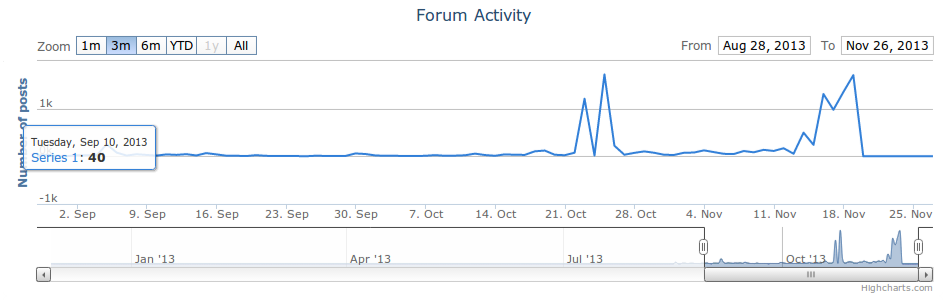
\includegraphics[width=0.5\textwidth]{images/activity.png}
\caption{A screen shot of activity measure graph.\label{fig:activity}}
\end{figure}

\subsubsection{Sentiment}

For every comment that came in, every word of the comment was separated in order to analyze them on their own.
Each word was assigned a sentiment score as per the document handed out in this class for assignment 1
known as AFINN-111. This document has a variety of English language words with scores assigned to them
between -5 and +5. If a word is assigned a negative score then that means it has negative sentiment (sad, 
angry, etc.) and if it has a positive score it has a happy sentiment. As per the comments, each word is assigned
a score and the total score for the comment is the aggregation of word scores within the comment. This final
score is also clamped between the values of -5 and +5 to avoid single comments skewing the results of
final analysis techniques. 

The results of the sentiment analysis is shown in Figure~\ref{fig:sent}. If no topic is specified, all comments
are used in the total sentiment analysis. If however, a user uses the search bar to provide a topic, only those
comments containing that topic are used.

\begin{figure}[h]
\centering
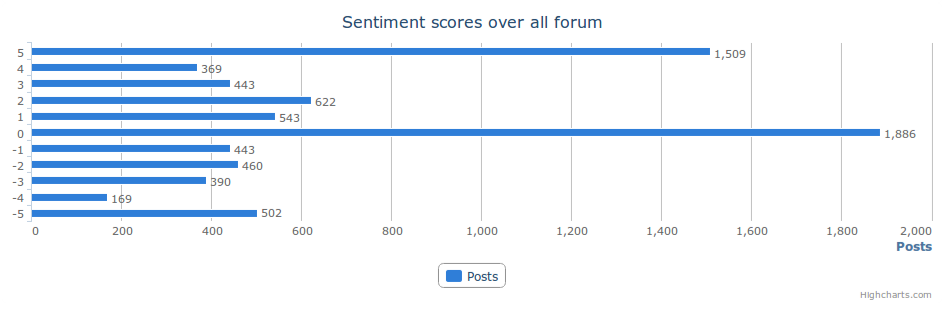
\includegraphics[width=0.5\textwidth]{images/sent.png}
\caption{A screen shot of sentiment measure graph.\label{fig:sent}}
\end{figure}

\subsubsection{Related Topics}

When a user searches for more information about a particular topic on the forum, FM presents them with related
topics to their search terms. In order to accomplish this, I used the python library called ``Topia''. Topia 
uses Parts of Speech in order to categorize every word from every post as noun, adjective, verb, etc. Once these
categorizations are completed, I simply filtered the words on nouns, objects, and verbs. This subset became the
list of topic words for any given comment. Once these keyword topics had been extracted, it was a simple algorithm
of seeing which keywords are referenced the most with the user provided topic. I ended up limiting it to the
top 50 keywords so as to not overwhelm the user. I found that the top 10 keywords ended up being the same for most
topics provided by the user, but the related topics ranked 10th - 30th were often quite useful. The related topics
can be seen in Figure~\ref{fig:rel}

\begin{figure}[h]
\centering
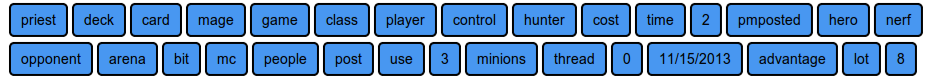
\includegraphics[width=0.5\textwidth]{images/rel.png}
\caption{A screen shot of related topics tags.\label{fig:rel}}
\end{figure}

\subsubsection{Requirements}

When a user searchers for more information about a particular topic, FM will present a list of requirements
as designated by the community surrounding that topic. In Figured~\ref{fig:req}, we can see that when
the user searchers for the term Priest, objects that are related to the Priest object in the game come up
with their recommended requirements.

\begin{figure}[h]
\centering
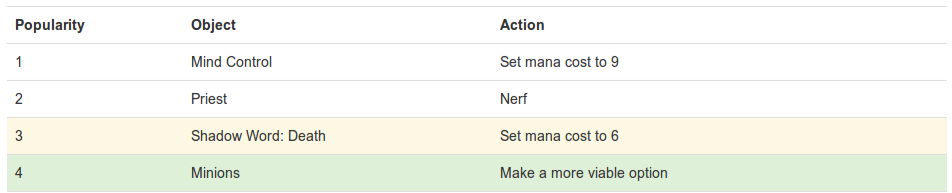
\includegraphics[width=0.5\textwidth]{images/req.png}
\caption{A screen shot of related topics tags.\label{fig:req}}
\end{figure}

The results seen in Figured~\ref{fig:req} are hard coded for this example as the actual algorithm implemented
was not quite as good as was expected (I will address this in Section~\ref{sec:fw}). In order to achieve these
results, I followed the following algorithm. First I found which keywords were related to the search term as
seen in the related topics section above. Once I had these, I found which sentences in which posts correlated
to these topic discussion. I then used ``Topia'' once again in order to label the Parts of Speech found in
the sentences. I then extracted the objects and verb phrases of the sentences. For instance, the sentence 
``I think that Mind Control is too strong and that it should be set to 9 mana.'' will have extracted
Mind Control as the object and set to 9 mana as the verb phrase. This was my initial idea for the requirements
algorithm, however it yielded very difficult to read output and require myself to intervene and make the
results readable, in terms of sentence structure, to other users. I have plans to improve this algorithm
which I will talk about in Section~\ref{sec:fw}.

\subsection{Visualization}

In order to visualize all of the previous analysis techniques, I used a variety of tools. I first used Ruby
on Rails in order to create a web application to host all of my findings. Ruby on Rails allows for quick prototyping
of website so it was an easy selection for this project.

I next had to find a way to graph both the sentiment and activity analysis I performed. I originally had planned
to use Google Charts as I had used them before in other big data applications, but I actually stumbled across
HighCharts.js, which is a great charting application for big data. HighCharts.js is a native only JavaScript
charting program which only requires jQuery (added in most projects anyways). This lack of dependency made it
an easy tool to work with. 

Finally, for styling purposes, I used Twitter's Bootstrap CSS framework. Bootstrap is used in many web applications
for its ease of use and for its polish.

\section{Future Work}
\label{sec:fw}

For the future work of this project, I really only have one major focus, but due to the nature of web applications,
other interesting additions can be created with ease. My main focus moving forward is in the further development
of the requirements elicitation tool. As per Figure~\ref{fig:req}, we can see how automatically generated
requirements may becomes handy to developers in that they can see what the community wants. However, finding 
these requirements and displaying them in a way that makes sense is difficult as found with this project.

In order to improve the requirements I suggest 2 steps. First to make the results more human readable, I would
like to incorporate other factors of the source sentences aside from object and verb phrase in order to make
the results a more cohesive sentence. Second, I would like to use some of the ideas from plagiarism detection
software and research in order to rank the findings better. Plagiarism research deals with taking two pieces of
English, say two sentences, and determining how alike they are. I would use this idea to find similar requirements.
If I can find requirements that are talked about by 90\% of the community, they are probably more high end priorities
for developers than a single suggestion by one user.

Through these two changes, I hope to make Forum-Miner a more robust tool and to eventual support community manager
jobs for software development.

\section{Conclusions}
\label{sec:conc}

This paper has walked through the creation and implementation of the ``Forum-Miner'' web tool. I have shown
how through the use of Python and web crawling, storage facilities, and Ruby on Rails, how we can create tools
which can perform deep analysis on natural unstructured data
that is available on the web through software system forums. Moving forward, I do not only hope to improve my
website by the better implementation of the requirements gathering algorithm, but I also hope to open the ideas
of this paper to further unstructured data research on the web. Free text is all over the place on the Internet,
but we do not yet have the tools to harness it.

I hope to release ``Forum-Miner'' to a public web server near April 2014 as I will be continuing this project
as a directed studies in the following semester. The code is available on GitHub.

% End of the paper
\end{document}
